Como se indicó en la introducción de esta memoria, el proyectante comenzó las
labores de ejecución del proyecto durante unas prácticas de empresa, antes de
decidir que se convertiría en su Proyecto Fin de Carrera. Es por ello que no se
hizo un \textit{Documento de Objetivos del Proyecto} ni un \textit{Plan de
Trabajo}.

En cambio, sí ha sido posible documentar con detalle cuál fue la evolución del
desarrollo del proyecto ya que, siguiendo la metodología de la empresa en la
que se realizó el desarrollo, se llevaba un registro diario de las actividades
realizadas.

El calendario se ha dividido en varias partes, siguiendo el proceso de trabajo
dividiéndolo en varias fases. Puede apreciarse que hay un periodo de
inactividad entre enero y febrero de 2011, entre la clasifcación de
\textit{bugs}, sugerencias... y la última recodificación. Este periodo
pertenece a una indisponibilidad por motivos familiares que, por suerte, no ha
resultado en retrasos con consecuencias mayores.

A continuación se describen de forma básica las acciones realizadas
por el proyectante en cada fase de desarrollo desde de que este comenzase allá
por junio de 2010 hasta que se depositó finalmente en junio de 2011. 

\section{Dirección del proyecto}

Se han incluido en esta sección todas las
actividades relacionadas con la comunicación con el cliente y el tutor del
proyecto.

\subsection{Comunicación con el cliente}

La primera reunión con el cliente para tratar específicamente el desarrollo de
este proyecto se llevó a cabo el 18 de junio de 2010, cuando el proyectante
llevaba realizando prácticas en la empresa un mes exactamente. Se trató la
necesidad del cliente, detallada en la sección \ref{sec:necesidad} (página
\pageref{sec:necesidad}), pero no la posibilidad de que esas labores se
convirtieran en su PFC.
La comunicación con el cliente ha sido constante a lo largo de todo el
proyecto, una característica que ha hecho posible que tanto desde el punto de
vista del proyectante como del cliente, el proyecto haya sido un éxito. Si
bien, al contrario de como se debía, no se elaboraron documentos específicos
acerca de la planificación, análisis... de cada parte, estos fueron sustituidos
por una comunicación constante, prácticamente diaria, con el cliente, que ha
supervisado la evolución del proyecto cada vez que su avance permitía ver
nuevos resultados o realizar nuevas pruebas. Cualquier no conformidad se
resolvía, con esta metodología, de manera casi inmediata, de manera que las
replanificaciones han sido, con alguna excepción no trivial, mínimas.

\subsection{Comunicación con el tutor}

Los primeros contactos con Ángel Luis Rubio, tutor de este proyecto, se
llevaron a cabo en septiembre de 2010 vía correo electrónico, y culminaron con
una primera reunión el 25 de octubre en la que se revisó lo hecho hasta el
momento y se concluyó que el reto que planteaba el desarrollo del proyecto
era adecuado como PFC, ni demasiado simple ni demasiado complejo.

Posteriormente, el contacto continuó a través de correo electrónico, con otra
reunión presencial el 11 de abril para resolver algunas dudas del proyectante
acerca de la organización y elaboración de la presente memoria.

\section{Módulo de personal}

Sin ánimo de adelantar detalles que corresponden a los próximos capítulos,
el módulo de personal fue la primera parte que se desarrolló. Se completó antes
de iniciar cualquier tipo de análisis de los módulos subsiguientes. La razón,
en un primer momento, era que el cliente pudiera confirmar la habilidad del
proyectante para completar un proyecto del alcance que ha llegado a tener. Así,
se llevó a cabo un gestor de personal cuyo funcionamiento interno se integra
apropiadamente con la base de datos existente y que es capaz de realizar todas
las funciones que necesitaba el cliente.

Este desarrollo se extendió desde la primera reunión con el cliente, en junio
de 2010, hasta mediados de agosto, en ratos libres dentro de las horas de
prácticas de empresa. La secuencia de actividades puede verse en el diagrama de
Gantt al final de este capítulo.

En resumen, las especificaciones principales
se definieron en una primera reunión con el cliente, a la que siguió un
esfuerzo por parte del proyectante de detección de entidades y diseño de la
base de datos que serviría de soporte lógico de almacenamiento de los datos.
Posteriormente, otra vez de acuerdo con el cliente, se realizaron una serie de
bocetos para la interfaz de usuario que se concretarían con el marcado HTML y
CSS, para continuar con la codificación de las funciones relativas a la gestión
del personal.

Una vez completado el desarrollo, el cliente revisaría el módulo para confirmar
que cumplía las especificaciones, y todo el \textit{feedback} sirvió para
mejorar la experiencia del usuario en una última fase de recodificación que,
por que el lector se haga una idea, añadió pequeños detalles como la posibilidad
de que al añadir datos anuales a un empleado, se tomasen por defecto los datos
del año anterior.

\section{Módulo de actividades}

Con un concepto similar al módulo de personal, se completó el
gestor de actividades antes de plantear la última fase de desarrollo
propiamente dicho. Así, siguiendo el mismo esquema de actividades que en la
sección anterior, las labores se extendieron desde mediados de agosto de
2010 hasta finales de septiembre.

Debe aclararse que la adición de la gestión de horas exige algunas pequeñas
modificaciones en la forma en que se presentan los datos relacionados con el
personal y las actividades, pero esas labores se han incluido en la siguiente
fase, no como recodificaciones de las mismas.

\section{Módulo de gestión de horas e integración}

Esta última parte del desarrollo fue la más complicada, pero gracias a la
experiencia adquirida en las fases anteriores, fue posible completarla con un
esquema de tiempos similar. Incluye la integración de todas las partes, ya que
a pesar de haber realizado desarrollos separados, las tres están íntimamente
relacionadas.

\section{Buscador global}

El buscador se desarrolló de forma más independiente, ya que fue una propuesta
del proyectante. Su desarrollo se llevó a cabo en ratos libres durante un
periodo de tres semanas, una vez se hubo implementado el módulo de personal.
Lo único que se añadió a posteriori fue un enlace de interés a las actividades
de los clientes y los proyectos, que son las dos entidades que se pueden
buscar, junto con los recursos. De cualquier modo, los detalles acerca del
buscador se pueden consultar en las secciones correspondientes de la presente
memoria.

\section{Última recodificación}

Apenas un mes después de que la herramienta comenzase a utilizarse en casos
reales y actuales y se hubieran reunido algunas sugerencias de modificación,
el proyectante sufrió una indisponibilidad familiar entre enero y febrero de
2011, periodo durante el cual cesó cualquier actividad del proyectante en
relación con la herramienta. Sin embargo, Ingeniería e Innovación siguió
utilizando el sistema sin mayores problemas y las mejoras que surgieron, todas
menores --más acerca de la usabilidad que de la funcionalidad--, fueron
implementadas en esta última etapa de codificación, que incluyó,
principalmente, hacer visible más resúmenes de los datos que ya estaban en la
base de datos y corregir algunos detalles relativos a la colaboración de
clientes en proyectos.

\section{Memoria y defensa}

Esta memoria comenzó a escribirse a mediados de abril del 2010, con la fecha de
finalización que aparece en la portada (el límite para su depósito fue el 17 de
junio). Como se ha indicado anteriormente, la forma en que se ha llevado a cabo
una vez finalizada la parte técnica del proyecto.

Por su parte, la fecha prevista para el inicio de la preparación para la
presentación y defensa del proyecto es mediados de junio, una vez finalizada
esta memoria completamente.

\begin{figure}[h]
\centering
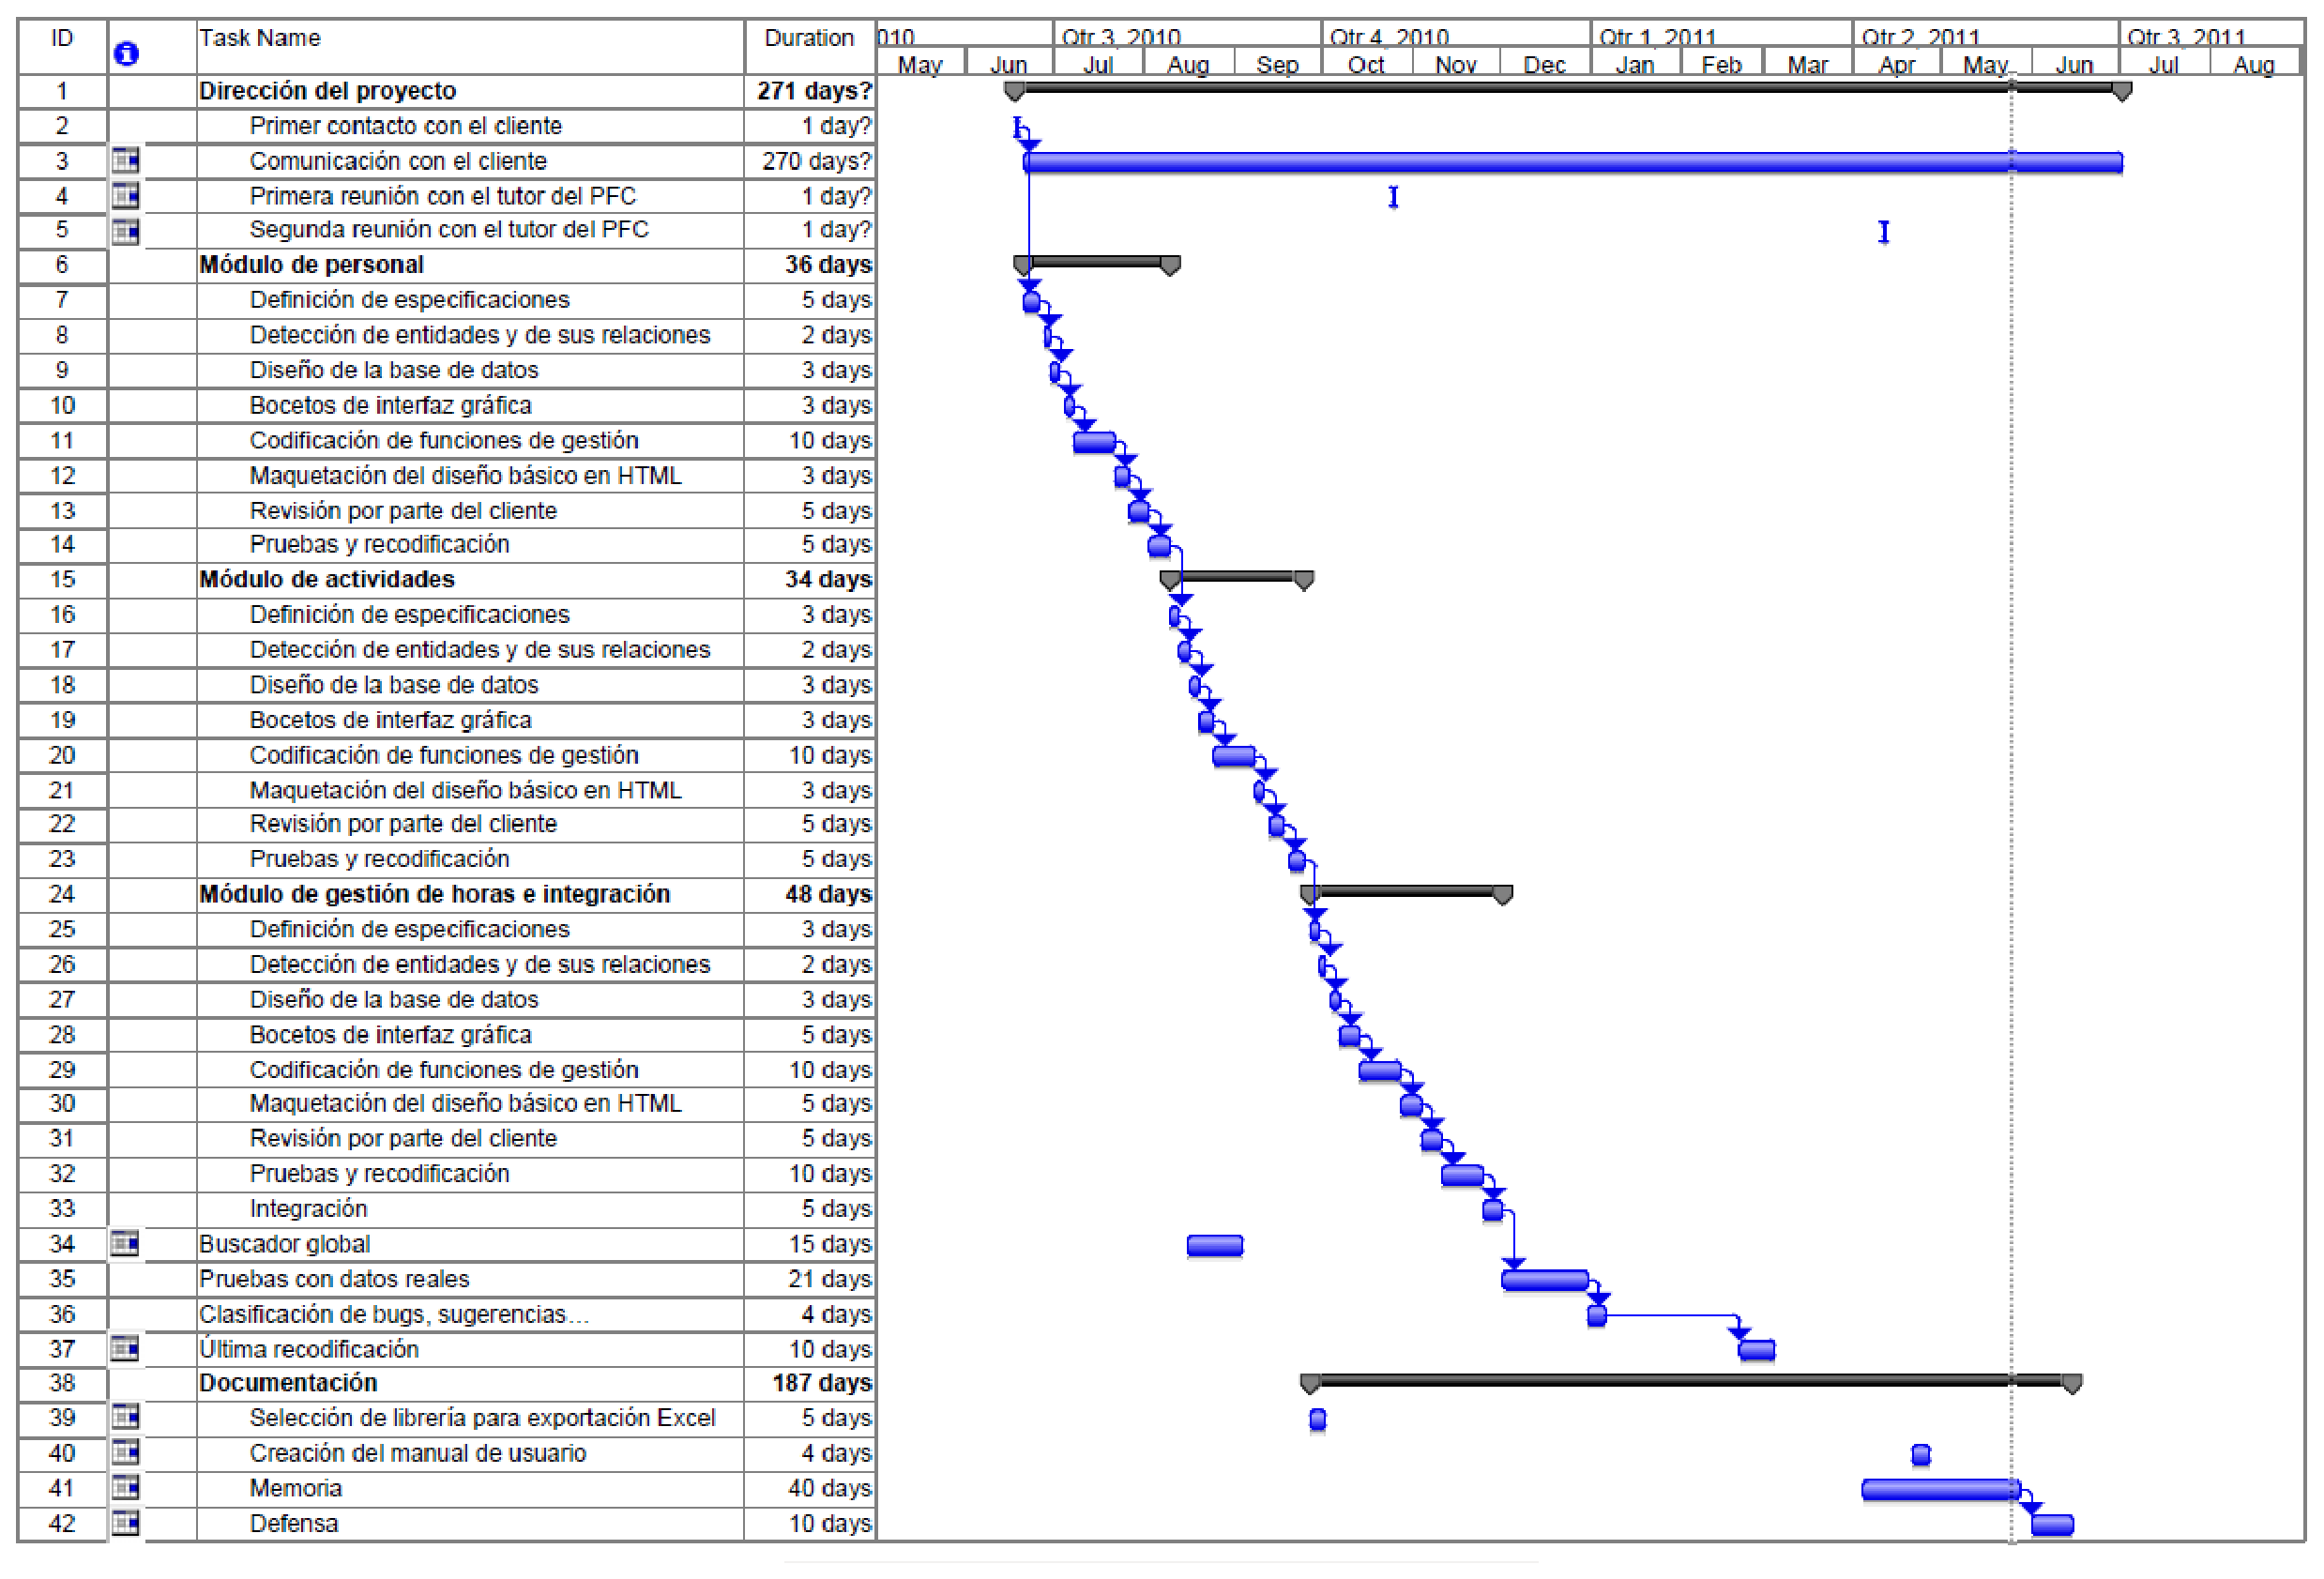
\epsfig{file=imagenes/gantt.eps,width=5.28in}
\caption{Diagrama de Gantt.}
\label{fig:gantt}
\end{figure}

%%%%GANTT
% {\linespread{1} \vfill\newpage
% \newsavebox{\myboxa}
% \sbox{\myboxa}{
% \begin{minipage}[t]{\textheight}
% \quad \vspace*{10pt}
% 
% 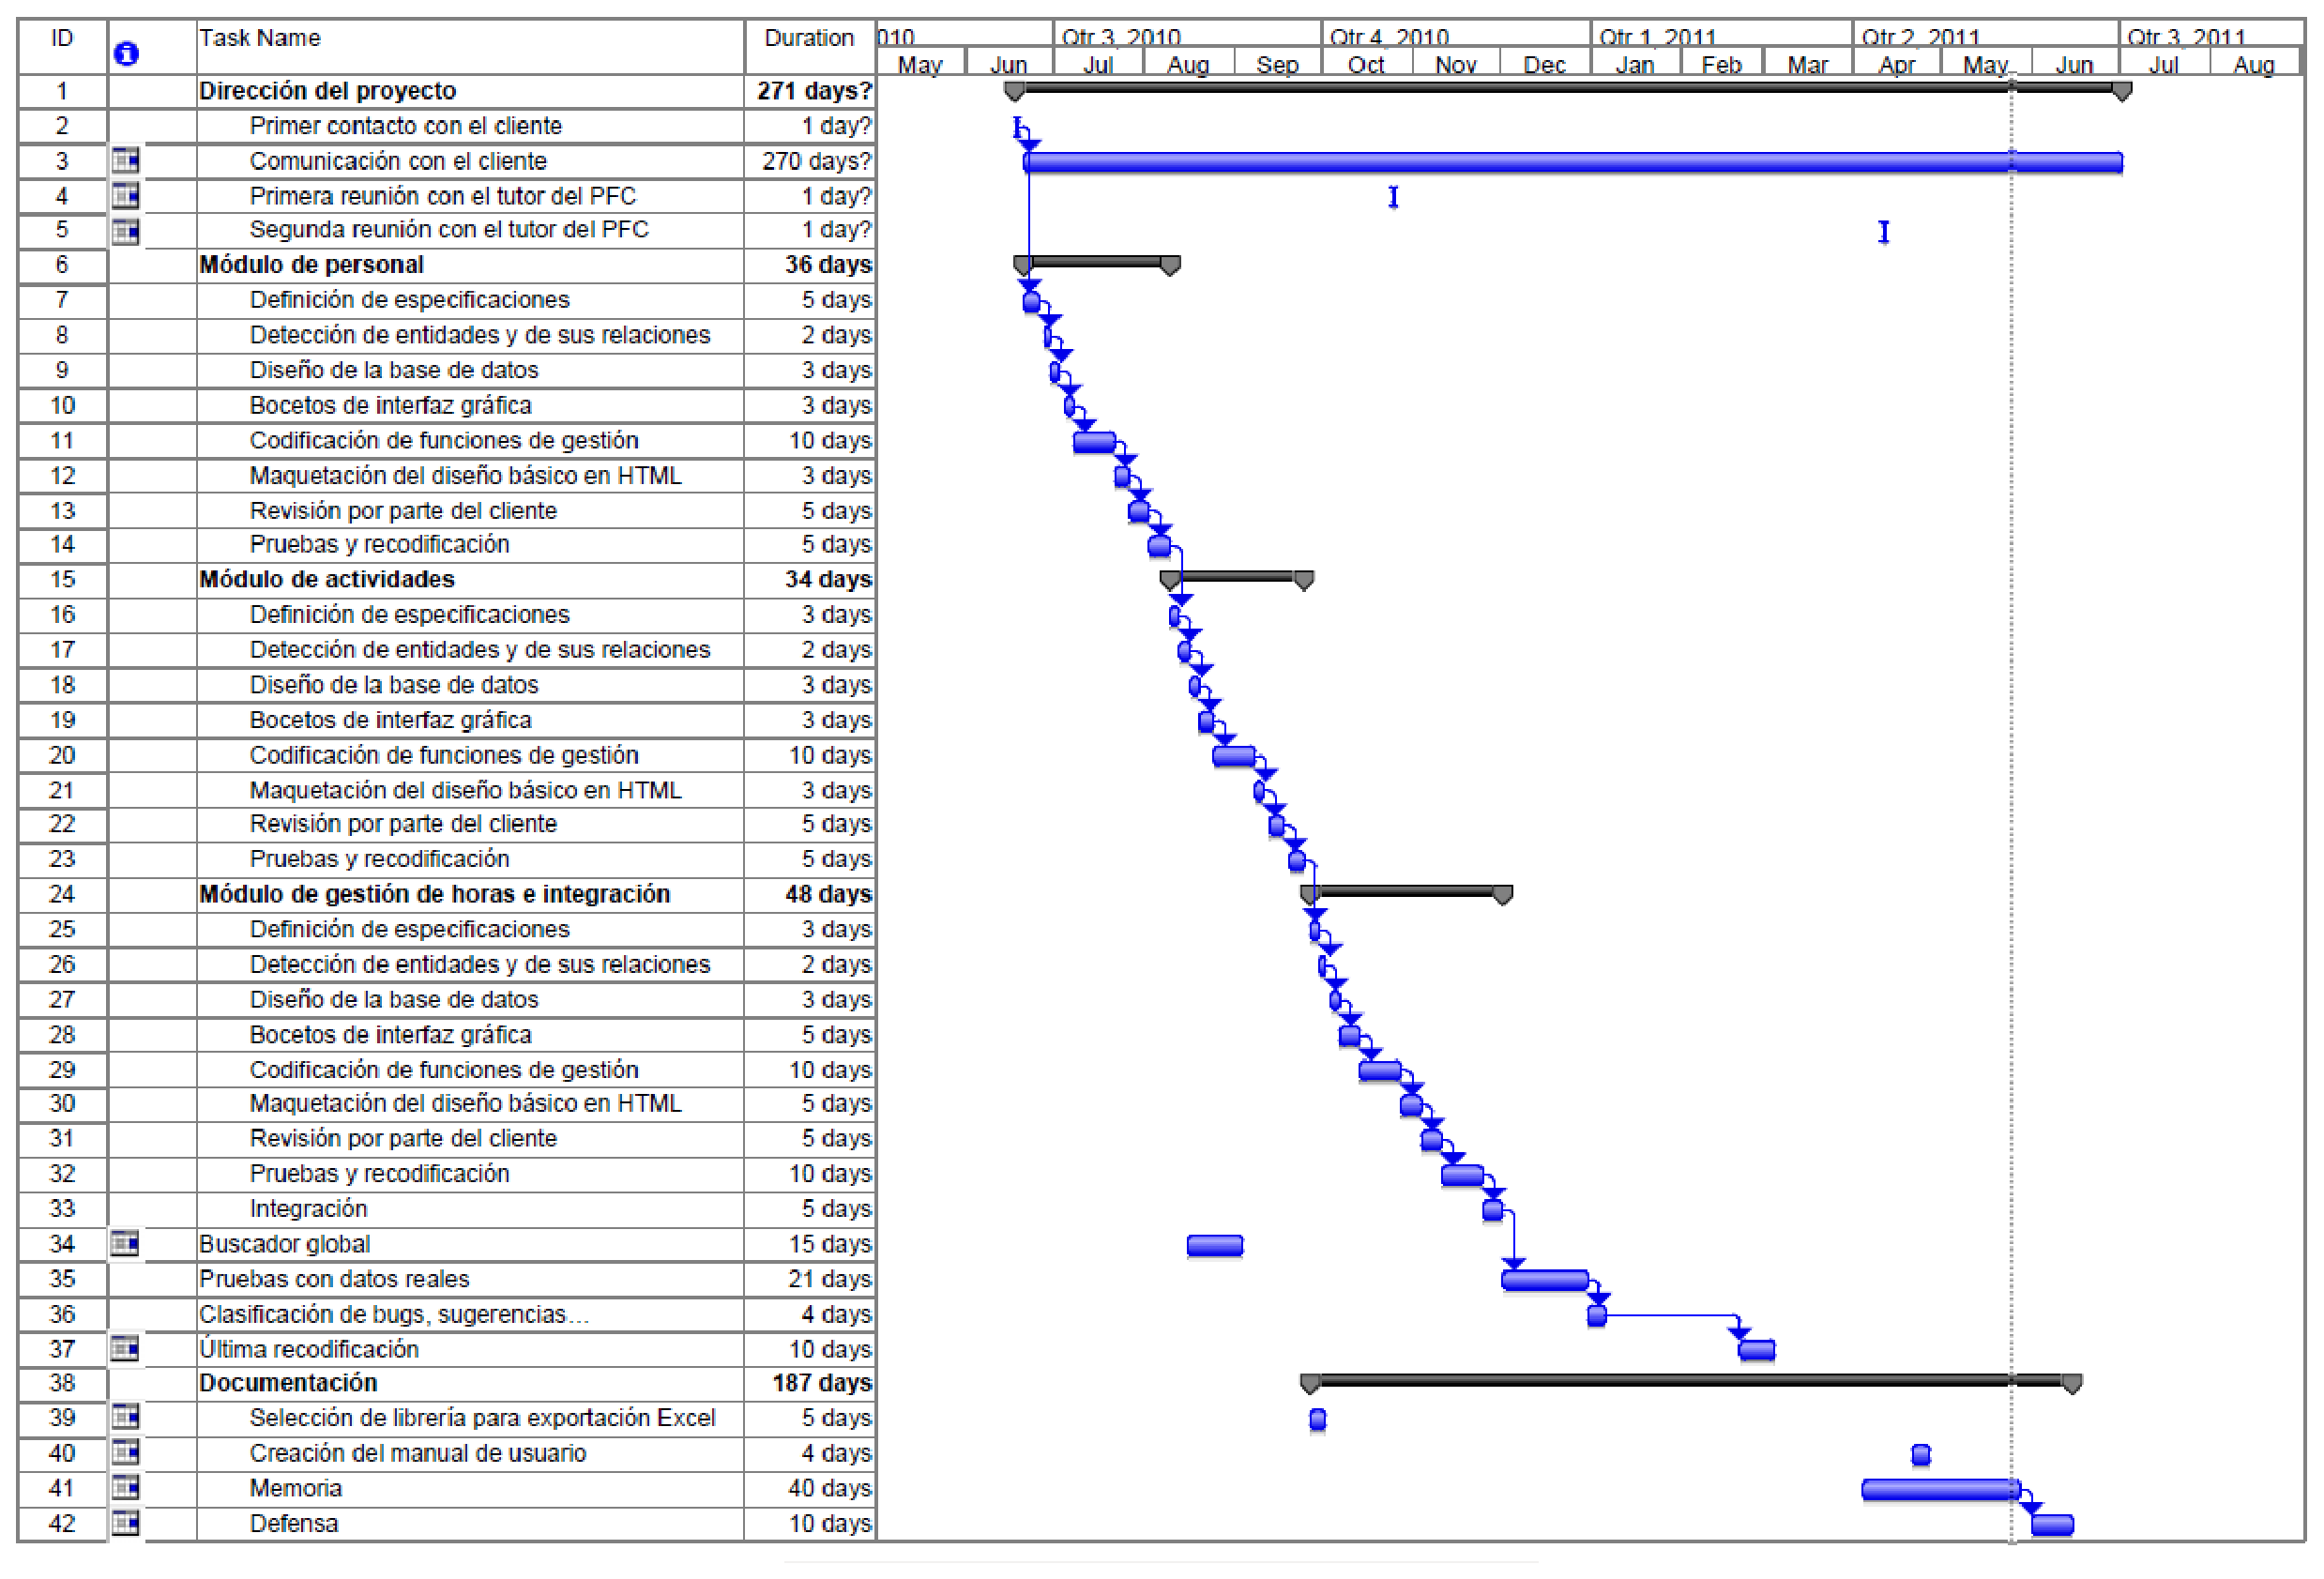
\epsfig{file=imagenes/gantt.eps,height=5in}
% 
% \end{minipage}
% } \quad\vfill \turnbox{90}{\usebox\myboxa}}
%%%%%%%%%%%%%%%%%%%%


 